% Summer research report: two-particle Hamiltonian system
% Restructured 2026-11-18 with f(E) as the only main line; periodic orbits,
% the E=52 section and the example cases moved to the appendices.
% Earlier versions:
%   report/archive/report_2026-11-07_before_simplify.tex
%   report/archive/report_2026-11-18_before_restructure.tex
%   report/archive/report_2026-11-18_before_fE_mainline.tex
%   report/archive/report_2026-11-18_before_user_edits.tex
% Data sources: report01-04.ipynb, case3_newton_failure_diagnosis.ipynb,
% lyapunov_*.py, regular_fraction_scan.py; figures from the scripts listed in
% the README of the repository.
% Text marked with \todo{...} still needs checking or a decision.

\documentclass[11pt,a4paper]{article}

\usepackage[margin=2.5cm]{geometry}
\usepackage{amsmath,amssymb}
\usepackage{graphicx}
\usepackage{booktabs}
\usepackage{xcolor}
\usepackage[colorlinks=true,linkcolor=blue!50!black,citecolor=blue!50!black,urlcolor=blue!50!black]{hyperref}

\graphicspath{{../images/}{figures/}}

% Figures and tables use [H] (float package): placed exactly where they are
% in the source, right after the paragraph that first refers to them.
\usepackage{float}

% Visible placeholder. For a clean draft use \newcommand{\todo}[1]{}
\newcommand{\todo}[1]{\textcolor{red}{[TODO: #1]}}

\newcommand{\q}{\mathbf{q}}
\newcommand{\p}{\mathbf{p}}
\newcommand{\Vs}{V_{\mathrm{sym}}}
\newcommand{\Eeq}{E_{\mathrm{eq}}}

\title{Regular and Chaotic Motion of Two Repelling Particles in a Box:\\
a Numerical Study}
\author{Jiajun Wu\\[2pt]
\small Department of Mathematics, Imperial College London\\
\small Summer research project (2026), supervised by Prof.\ Dmitry Turaev}
\date{November 2026}

\begin{document}
\maketitle

% ---------------------------------------------------------------------------
\begin{abstract}
We study numerically two particles in a square box that repel each other and
are pushed back by the walls, restricting to motions that are symmetric about
the centre of the box. We measure the fraction $f(E)$ of the energy surface
filled by regular motion, using finite-time Lyapunov exponents for initial
conditions sampled uniformly on the energy surface. Near the bottom of the
four potential wells all sampled trajectories are classified as regular. As the energy approaches
$E_s\approx1.9969$, the energy of the saddles between the wells, chaos
appears, and around $E_s$ the regular fraction drops sharply, to about $4\%$
at $E\approx2.05$; it then rises, quickly at first and then slowly, to about
one third at $E=200$. So
regular motion does not take over at high energy, at least up to $E=200$. We
explain the drop near $E_s$ by the low saddles between the wells, and at
$E\approx52$ we show that the regular motion forms islands around stable
periodic orbits, including one of the type studied by Rom-Kedar and Turaev.
\end{abstract}

% ---------------------------------------------------------------------------
\section{Introduction}\label{sec:intro}

Two particles that repel each other inside a box form a very simple system,
but their long-time motion is not obvious. They might settle into a repeating
pattern, or move chaotically over the whole box, depending on the energy and
the initial condition.

Rom-Kedar and Turaev \cite{turaev2022} proved that, under mild conditions,
the motion of $N$ repelling particles in a bounded region is not ergodic at
sufficiently high energies. They construct stable periodic orbits that are
surrounded by a set of positive measure of quasi-periodic motions; trajectories
that start in this set stay near the periodic orbit for all time, so they
cannot explore the whole energy surface. For particles in a rectangular box,
the stable orbit they construct is one in which every particle moves fast in
the same direction, say vertically, each on its own line and in synchrony with
the others \cite[Sec.~2.6]{turaev2022}. Their result is asymptotic: it holds
only above some energy that is not given explicitly, and it needs the wall
potential to be steep enough (Appendix~\ref{app:vertical}).

In this project we study numerically the simplest case, two particles in a
square box, restricted to motions that are symmetric about the centre. We ask
one question: how does the fraction of regular motion on the energy surface
depend on the energy? One might expect regular motion to dominate at both
ends: near the equilibrium, where the motion is a small oscillation, and at
high energy, where the particles move almost like billiard balls in a square,
whose single-particle motion is integrable. We test this by measuring the
regular fraction $f(E)$ from the equilibrium up to $E=200$, and then explain
the shape of the curve.

Section~\ref{sec:model} describes the model and its potential landscape, and
Section~\ref{sec:methods} how we measure $f(E)$. Section~\ref{sec:results}
presents $f(E)$ and explains it at low and at high energy.
Section~\ref{sec:discussion} summarises the findings and their limitations.
The appendices contain the convergence checks and the supporting computations
of individual periodic orbits.

% ---------------------------------------------------------------------------
\section{The model}\label{sec:model}

Two particles with positions $\q_i=(x_i,y_i)$ and momenta $\p_i$ ($i=1,2$)
move in the box $(0,L_x)\times(0,L_y)$. The Hamiltonian is
\begin{equation}\label{eq:H}
  H(\q,\p)=\sum_{i=1}^{2}\frac{|\p_i|^2}{2m_i}
  + V\bigl(|\q_1-\q_2|\bigr) + U(\q_1) + U(\q_2),
\end{equation}
where
\begin{equation}\label{eq:potentials}
  V(r)=k\,r^{-\alpha},\qquad
  U(x,y)=C\Bigl[x^{-\beta}+(L_x-x)^{-\beta}+y^{-\beta}+(L_y-y)^{-\beta}\Bigr].
\end{equation}
$V$ is the repulsion between the particles and $U$ pushes each particle away
from the walls. Both become infinite at collision or at a wall, so the
particles can never collide or leave the box.

We take $k=C=\alpha=\beta=1$, $m_1=m_2=1$ and $L_x=L_y=10$. These are simply convenient values and the model is not meant to describe a specific physical system.

\paragraph{Symmetric motions.}
If particle~2 starts at the point reflection of particle~1 through the centre
of the box, $\q_2=(10,10)-\q_1$, with the opposite momentum $\p_2=-\p_1$,
then by symmetry this relation is preserved for all time. We call such
motions \emph{centre-symmetric}. For centre-symmetric motions, the positions and momenta of both particles are completely determined by those of particle 1, reducing the dynamics to a system with two degrees of freedom. Substituting the symmetry relations into~\eqref{eq:H}, the total energy becomes
\begin{equation}\label{eq:Hsym}
  H_{\mathrm{sym}}(\q_1,\p_1)=|\p_1|^2+\Vs(\q_1),\qquad
  \Vs(\q_1)=V\bigl(|2\q_1-(10,10)|\bigr)+2\,U(\q_1).
\end{equation}
Here $\Vs$ is the total potential energy of the centre-symmetric system.
All initial conditions in this report are chosen to be centre-symmetric.

\paragraph{Wells and saddles.}
Figure~\ref{fig:potential} shows $\Vs$. By the symmetry of the square it has
four equivalent minima, at $\q_1=(a,a)$, $(10-a,a)$, $(a,10-a)$ and
$(10-a,10-a)$ with $a\approx3.6645$, all with energy
$\Eeq\approx1.98765$; this is the equilibrium, with the particles at rest on a
diagonal of the box. Between neighbouring minima there are four saddles, at
$\q_1\approx(3.1926,5)$ and the three points obtained by symmetry, with energy $E_s\approx1.99689$. The
centre of the box, where the particles would collide, is a singularity. So the
bottom of the potential is a ring-shaped valley around the centre, with four
wells separated by saddles only $E_s-\Eeq\approx0.0092$ higher
(Figure~\ref{fig:potential}(d)). For $E<E_s$ the region $\{\Vs<E\}$ that
particle~1 can reach consists of four separate pieces, one around each
minimum; for $E>E_s$ they join into a ring (Figure~\ref{fig:potential}(b,c)).
% Values from images/make_potential_figure.py (2026-11-18): well Hessian
% eigenvalues 0.0228, 0.2454; saddle Hessian eigenvalues -0.0207, 0.3050.

% Generated by images/make_potential_figure.py
\begin{figure}
  \centering
  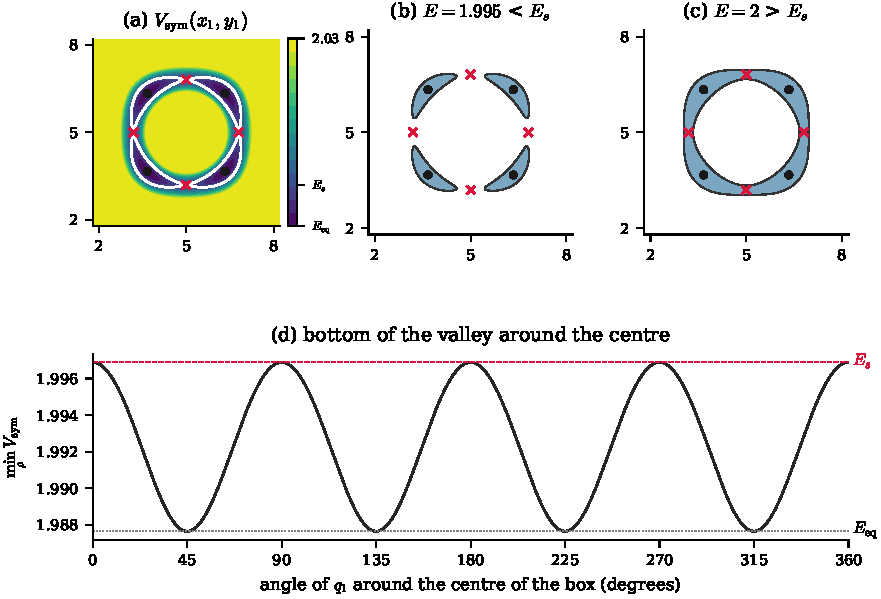
\includegraphics[width=\textwidth]{fig_potential.pdf}
  \caption{The potential $\Vs(\q_1)$ of a centre-symmetric motion. (a)
  Contours near the bottom; black dots are the four minima, red crosses the
  four saddles, and the white line is the level $\Vs=E_s$. (b), (c) The region
  $\{\Vs<E\}$ that particle~1 can reach just below and just above $E_s$.
  (d) The bottom of the valley, $\min_\rho\Vs$ along each ray from the centre,
  against the angle of the ray.}
  \label{fig:potential}
\end{figure}

% ---------------------------------------------------------------------------
\section{Measuring the regular fraction}\label{sec:methods}

\subsection{Time integration}
For centre-symmetric motions, we integrate the equations of motion
of particle~1, with particle~2 determined by symmetry, using the
leapfrog method:
\begin{equation}\label{eq:leapfrog}
  \p^{n+1/2}=\p^n+\tfrac h2 F(\q^n),\quad
  \q^{n+1}=\q^n+h\,\p^{n+1/2},\quad
  \p^{n+1}=\p^{n+1/2}+\tfrac h2 F(\q^{n+1}).
\end{equation}
Here $\q=\q_1$ and $\p=\p_1$, and
$F=-\frac12\nabla\Vs$ is the force on particle~1,
as inherited from the original two-particle equations of motion.
The time step is $h$. Leapfrog is a second-order symplectic method with good long-time energy behaviour \cite{hairer2006}, which is important because we integrate for up to
$2\times10^4$ time units. The particles move faster at higher energy, so we
take $h=\min\bigl(5\times10^{-3},\,0.026/E\bigr)$, which keeps the relative
energy error below $6\times10^{-4}$.
% Scan: max|dE|/E = 1.7e-4 (E=10), 1.6e-4 (E=52.23), 6.4e-4 (E=200).

\subsection{Regular or chaotic: the Lyapunov exponent}\label{sec:lyap-method}
The Lyapunov exponent $\lambda_{\max}$ of a trajectory measures how fast two
nearby trajectories separate: it is $0$ for regular motion and positive for
chaotic motion \cite{lichtenberg1992}. We estimate it by following, along the trajectory, a small
perturbation with the linearised leapfrog map, renormalising it every 40 steps
and averaging the logarithm of its growth over a time $T$. The perturbation is
kept centre-symmetric, so $\lambda_{\max}$ measures instability within the
centre-symmetric motions only.

To decide whether a trajectory is regular we need a threshold for the
finite-time estimate $\lambda_T$. For a regular trajectory nearby trajectories
separate only linearly in time, so $\lambda_T$ is not exactly $0$ but of order
$\ln T/T$, and it decreases as $T$ grows. For a chaotic one they separate
exponentially, and $\lambda_T$ tends to a positive constant. We therefore call
a trajectory \emph{regular} if
\begin{equation}\label{eq:threshold}
  \lambda_T < c\,\frac{\ln T}{T},\qquad c=3.2 .
\end{equation}

To see whether the result depends on $c$, we looked at the values of
$\lambda_T$, in units of $\ln T/T$, for all trajectories of the
regular-fraction scan of Section~\ref{sec:fraction-method}: $3600$
trajectories at each of $23$ energies from $E=1.99$ to $200$.
At most energies only very few trajectories (at most $2.5\%$) have
$\lambda_T$ between $2\ln T/T$ and $5\ln T/T$, so any $c$ between $2$ and $5$
gives almost the same classification; Figure~\ref{fig:threshold} shows this
gap at three energies. The exception is $E=1.995$--$1.997$, just below and at
$E_s$, where the chaos is weakest, with up to $9\%$ of the trajectories in the
gap. We take
$c=3.2\approx\sqrt{2\cdot5}$, the middle of the gap on the logarithmic scale.
% Statistics from images/make_threshold_figure.py (standard T, 2026-11-18):
% fraction with 2<u<5: <= 0.025 except E=1.995 (0.078), 1.996 (0.094),
% 1.997 (0.033).

% Generated by images/make_threshold_figure.py
\begin{figure}[H]
  \centering
  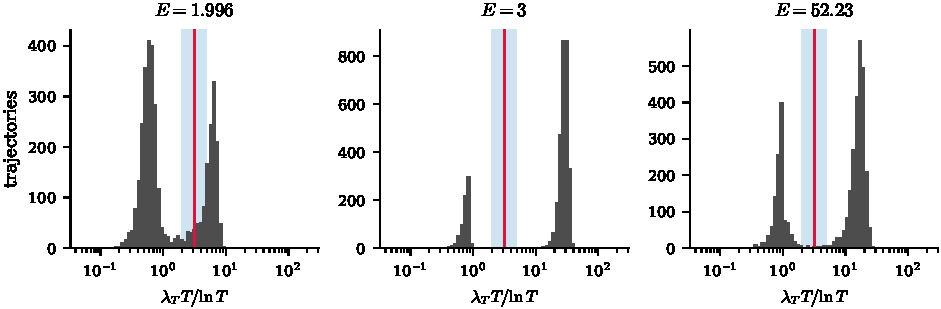
\includegraphics[width=\textwidth]{fig_threshold.pdf}
  \caption{Histograms of $\lambda_T$ in units of $\ln T/T$ for the $3600$
  trajectories of the regular-fraction scan at three energies.
  The left group is regular, the right group chaotic. Red line: the threshold
  $c=3.2$; blue band: $2\le c\le5$.}
  \label{fig:threshold}
\end{figure}

\subsection{Sampling the energy surface}\label{sec:fraction-method}
We define the regular fraction $f(E)$ as the fraction of the energy surface
$\{H_{\mathrm{sym}}=E\}$, measured with the Liouville (microcanonical)
measure, that is filled by regular trajectories. To estimate it we sample
initial conditions from this measure, integrate each one and count the regular
ones. We draw $\q_1$ uniformly from the accessible region $\{\Vs<E\}$, the
direction of $\p_1$ uniformly from $[0,2\pi)$, and set
$|\p_1|=\sqrt{E-\Vs(\q_1)}$. We use $3600$ trajectories per energy.

For $E>2.05$ the integration time is chosen so that every energy gets a
similar number of wall-to-wall flights:
$T=\min\bigl(2500,\;500\sqrt{52.23/E}\bigr)$. For $E\le2.05$, near the
equilibrium and the saddles, the motion is a slow oscillation rather than a
flight between the walls, and the chaos is very weak: an orbit that looks regular may only reveal its chaos after many oscillations, so we integrate up to $T=10\,000$. Appendix~\ref{app:convergence} checks that these times are long enough.

% ---------------------------------------------------------------------------
\section{Results}\label{sec:results}

\subsection{Regular and chaotic trajectories}\label{sec:sections}
Before measuring how common regular motion is, we look at single
trajectories at a given energy. A convenient way to see the type of motion is a
\emph{Poincar\'e section}: we record $(x_1,p_{x_1})$ each time particle~1
crosses a chosen horizontal line $y_1=\mathrm{const}$ upwards. For a centre-symmetric
motion, $p_{y_1}$ then follows from the energy, so this section is exactly
two-dimensional. On it a regular trajectory gives points on
smooth closed curves, and a chaotic one gives points scattered over a
two-dimensional region \cite{lichtenberg1992}.

We start from the position $\q_1=(a,a)+0.25\,(1,1)$ near a minimum and give
the particles vertical momenta of increasing size
(Figure~\ref{fig:energy-sections}).
\begin{itemize}
  \item At $E\approx2.007$ the section points lie on smooth curves: regular
        motion.
  \item At $E\approx2.028$ and $E\approx2.97$ the points are scattered and the
        trajectory wanders over a large part of the box: chaotic motion.
  \item At $E\approx11$ the motion is regular again. The particles stay in two
        thin vertical strips, close to a stable vertical periodic orbit
        (Appendix~\ref{app:vertical}).
\end{itemize}

\begin{figure}[H]
  \centering
  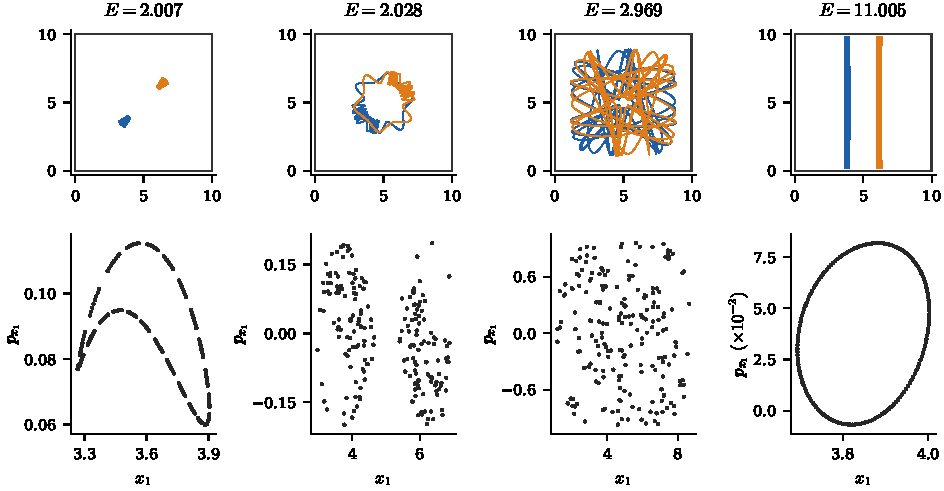
\includegraphics[width=\textwidth]{fig_energy_sections.pdf}
  \caption{Starting from $\q_1=(a,a)+0.25\,(1,1)$ with vertical momenta
  $\pm v$ at four energies: trajectories (top) and 200 returns to the section
  $y_1=a$, $p_{y_1}>0$ (bottom).}
  \label{fig:energy-sections}
\end{figure}

\subsection{The regular fraction}\label{sec:fraction}
Figure~\ref{fig:fraction} shows the regular fraction $f(E)$ at 23 energies
from $E=1.99$ to $E=200$. The curve has three stages.
\begin{itemize}
  \item Near the bottom of the wells all sampled trajectories are classified as regular ($f=1$).
  \item Around $E_s$, starting slightly below it, $f$ drops steeply, to a
        minimum of about $0.04$ at $E=2.05$.
  \item Above that, $f$ rises again, quickly up to $E\approx2.7$; after a
        dip at $E=3$, it then rises slowly, to about one third at $E=200$.
\end{itemize}
So the expectation of Section~\ref{sec:intro} holds near the equilibrium,
but it does not hold, up to $E=200$, at high energy.

% Generated by images/make_fraction_figure.py
\begin{figure}[H]
  \centering
  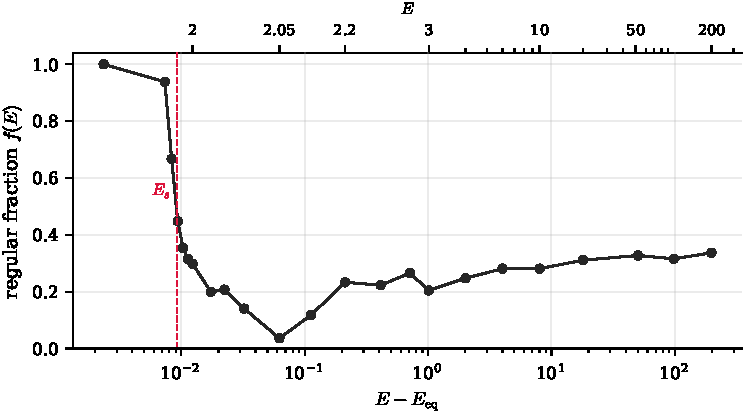
\includegraphics[width=0.8\textwidth]{fig_regular_fraction.pdf}
  \caption{Regular fraction $f(E)$ of the (centre-symmetric) energy surface,
  against $E-\Eeq$ (bottom axis) and $E$ (top axis), with the threshold
  $c=3.2$ of~\eqref{eq:threshold} and the integration times of
  Section~\ref{sec:fraction-method}. Each point uses $3600$ trajectories
  sampled uniformly on the energy surface. Dashed line: the
  saddle energy $E_s$.}
  \label{fig:fraction}
\end{figure}

\paragraph{Is $T$ long enough?}
With a finite $T$, a weakly chaotic trajectory may still look regular, so
$f$ may be too high. Doubling the integration time lowers $f$ by at most
$0.02$ for $E>2.05$ and by at most $0.044$ for $E\le2.05$, the largest
changes being just below $E_s$ (Appendix~\ref{app:convergence}). But these changes,
like those from the choice of threshold (Section~\ref{sec:lyap-method}), are
much smaller than the drop around $E_s$ and the slow rise above it, so the
general shape of the curve does not change.

\paragraph{Is $f$ still growing at high energy?}
From $E=10$ to $E\approx52$ the regular fraction clearly grows, from $0.28$
to $0.33$. Above that the values at $E\approx52$, $100$ and $200$ are
$0.328$, $0.316$ and $0.337$, which do not increase steadily, so from these
data we cannot tell whether $f$ is still growing slowly or has levelled off.
More energies above $E=52$ would be needed.

\subsection{Low energy: why $f$ drops near the saddles}\label{sec:transition}
Near the bottom of a well the potential is nearly quadratic,
so the motion is close to two independent harmonic oscillations,
which form an integrable system. This suggests that regular
motion should dominate at sufficiently low energies, consistent
with our observation that all sampled trajectories at $E=1.990$
were classified as regular.

As $E$ approaches $E_s$, the part of a well that particle~1 can reach extends
up to the saddles (Figure~\ref{fig:potential}(b)). Near a saddle the particle
moves slowly, and what it does next depends very sensitively on how it
arrives.
Motion near separatrices is a common source of chaos in
Hamiltonian systems \cite{lichtenberg1992}. This suggests
that chaotic motion may appear even slightly below the
saddle energy, consistent with our numerical observations. At $E=1.995$ and $1.996$ no trajectory leaves its well
(none crosses the line $y_1=5$), yet about $6\%$ and $33\%$ of them are
chaotic. Figure~\ref{fig:saddle-sample} shows nine trajectories at
$E=1.996$, picked at random. The four chaotic ones all run along the whole
well, up to both of its ends next to the saddles, while three of the five
regular ones stay near the bottom of the well. However, we have yet to check this systematically.

% Generated by images/make_saddle_sample_figure.py
\begin{figure}
  \centering
  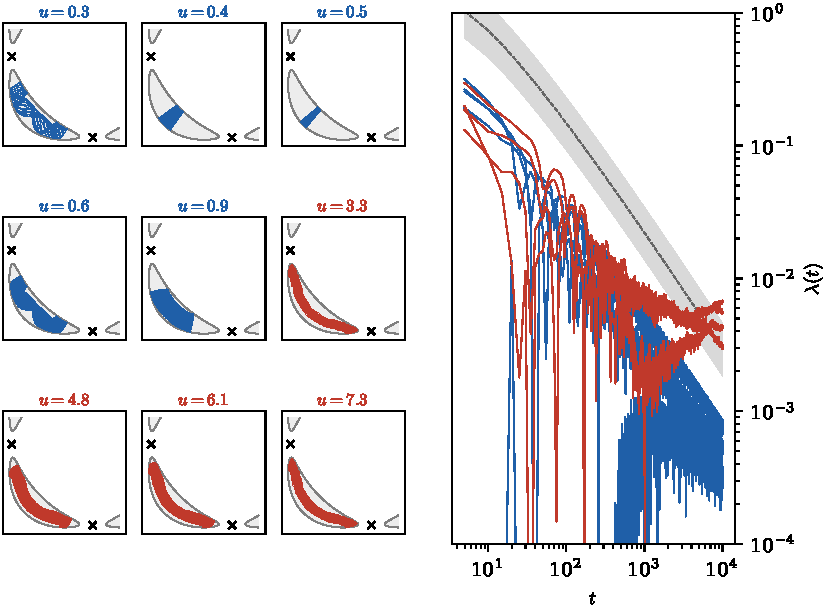
\includegraphics[width=\textwidth]{fig_saddle_sample.pdf}
  \caption{Nine trajectories at $E=1.996$, just below $E_s$, picked at random
  from $30$ sampled on the energy surface and integrated for $T=10\,000$.
  Left: particle~1 in its well, mapped into the lower-left well by the
  symmetry of the square; grey: the accessible region $\{\Vs<E\}$; crosses:
  the two saddles next to this well. Blue: regular, red: chaotic, with
  $u=\lambda_T T/\ln T$ (regular if $u<3.2$). Right: $\lambda_T$ of the
  same nine trajectories as a function of the integration time $T$; grey band:
  $2\ln T/T$ to $5\ln T/T$; dashed line: the threshold $3.2\ln T/T$.}
  \label{fig:saddle-sample}
\end{figure}

For $E>E_s$ particle~1 can pass over the saddles from one well to the next.
Because the barrier between the wells is so low,
$E_s-\Eeq\approx0.0092$, many trajectories can pass
between wells even when $E$ is only slightly above $E_s$.
These passages bring trajectories into the neighbourhood
of the saddles, where chaotic behaviour may occur. Indeed, as $E$ increases from $1.997$ to
$2.000$ and $2.05$, the fraction of trajectories that cross $y_1=5$, indicating passages between wells, grows from $34\%$ to $72\%$ and over $99\%$, while
$f$ falls from $0.45$ to $0.30$ and $0.04$.

\subsection{High energy: where the regular motion is}\label{sec:high}
As $E$ grows, the wells and saddles become less important compared with the
total energy. To see where the regular motion lies, we examine the Poincar\'e
section $y_1=5$, $p_{y_1}>0$ at $E\approx52.23$ (Figure~\ref{fig:lyapunov}).
This energy has no special meaning: it is the energy of the circular orbit
computed in Appendix~\ref{app:circular}. We included the same energy in the
scan of $f(E)$, so that the regular fraction found from the section can be
compared with the one found by sampling the energy surface.

We use a uniform grid of $13\,920$ initial conditions on the section,
integrated for $T=500$ with $h=10^{-3}$, and colour each point by the
finite-time Lyapunov exponent of its trajectory. The regular trajectories
form many islands inside a large chaotic region; the histogram of Lyapunov
exponents also shows two distinct groups.

The islands cover about $33\%$ of the section area, or $31\%$ when weighted
by return time to account for the measure on the energy surface. This is
broadly consistent with $f\approx0.33$ obtained by sampling the energy
surface directly with the same integration time.

% Generated by images/make_lyapunov_section_figures.py
\begin{figure}[H]
  \centering
  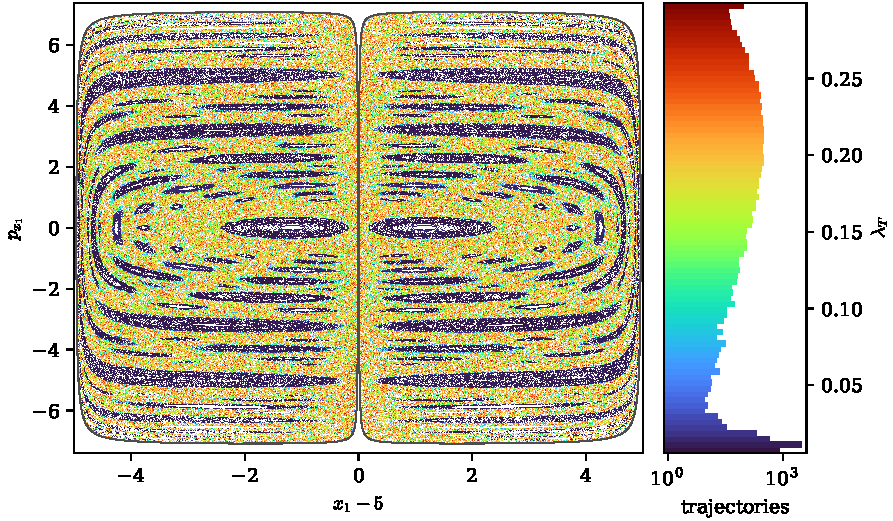
\includegraphics[width=\textwidth]{fig_lyapunov_section.pdf}
  \caption{Poincar\'e section at $E\approx52.23$, each point coloured by the
  finite-time Lyapunov exponent of its trajectory ($13\,920$ trajectories,
  $T=500$). Dark points (small exponents) form islands of regular motion
  within a chaotic region. Right: histogram of the exponents (number of
  trajectories on a logarithmic scale).}
  \label{fig:lyapunov}
\end{figure}

Using Newton's method, we found linearly stable periodic orbits at the
centres of several islands (Figure~\ref{fig:islands}). The simplest is the
\emph{vertical orbit}, in which the two particles move between the top and
bottom walls, each along its own nearly vertical path. This is the type of
orbit constructed by Rom-Kedar and Turaev for a rectangular box
\cite[Sec.~2.6]{turaev2022}. Their theorem does not apply to our wall
potential, but numerically this orbit is linearly stable at the energies
examined from $E\approx3.9$ upwards (Appendix~\ref{app:vertical}).
Another stable orbit has the particles moving around the centre of the box,
opposite each other. At high energy it approaches a diamond-shaped billiard
orbit, with turning points near the middle of each wall
(Appendix~\ref{app:circular}). The other periodic orbits shown in
Figure~\ref{fig:islands} have more complicated shapes. We have not measured
how much each island contributes to the regular fraction.

% Generated by images/make_lyapunov_section_figures.py
\begin{figure}
  \centering
  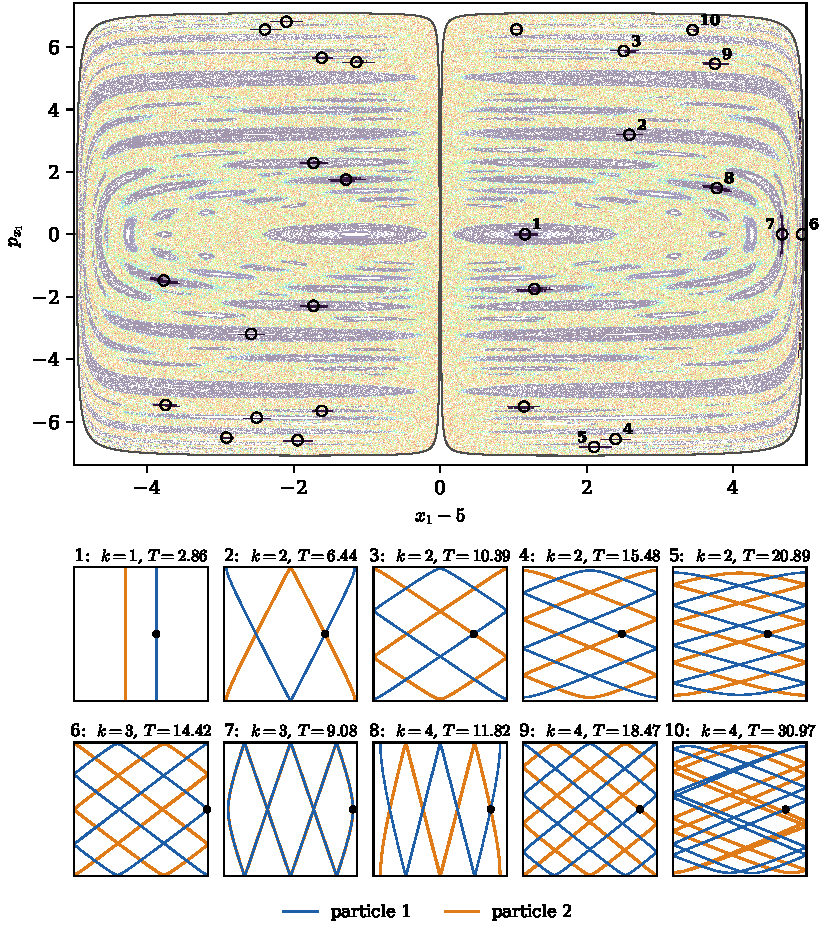
\includegraphics[width=\textwidth]{fig_islands.pdf}
  \caption{Ten linearly stable periodic orbits found at the centres of regular
  islands at $E\approx52.23$. Top: their points on the Poincar\'e section
  $y_1=5$, $p_{y_1}>0$ (circles). An orbit whose particle~1 crosses the line
  $y_1=5$ upwards $k$ times per period gives $k$ circles on the diagram, and only one of them is numbered. Black regions near circles: returns of trajectories started close to these points,
  which trace islands too small to be resolved by the grid of
  Figure~\ref{fig:lyapunov}. Below: the orbits in the box, with $k$ and the
  period $T$.}
  \label{fig:islands}
\end{figure}

% ---------------------------------------------------------------------------
\section{Discussion}\label{sec:discussion}

\paragraph{Summary.}
The regular fraction $f(E)$ has three stages. Near the bottom of the wells our sampled
trajectories are classified as regular, consistent with nearly harmonic motion. As the energy
approaches the saddle energy $E_s\approx1.9969$, trajectories can come close to
the saddles and chaos appears, already slightly below $E_s$; above $E_s$, when
particle~1 can move between the wells, chaos takes over almost the whole
energy surface, with a minimum $f\approx0.04$ at $E\approx2.05$. At higher
energy $f$ recovers, quickly at first and then slowly, to about one third at
$E=200$; this regular motion
lies on islands around stable periodic orbits. So regular motion dominates
only near the equilibrium.

\paragraph{Relation to Rom-Kedar and Turaev.}
Our results agree with their picture that stable periodic orbits keep the
motion from being ergodic, at least within the centre-symmetric motions:
the regular fraction stays positive at all energies we computed, and at
$E\approx52$ we checked that the regular trajectories lie on islands around
linearly stable periodic orbits. In addition, we measured how the regular
fraction depends on the energy, which their theorem does not address.

\paragraph{Limitations.}
All results are for centre-symmetric motions. These form a
four-dimensional subset of the eight-dimensional phase space, of zero
volume, so the regular fraction we measure is a fraction of the symmetric
energy surface, not of the full one, and the islands we see are islands of
the symmetric system. The Lyapunov exponents are computed over a finite
time, so very weak chaos may be counted as regular, and the classification
depends on a threshold; we checked both effects but cannot remove them.

\paragraph{Open questions.}
\begin{itemize}
  \item Does $f(E)$ keep growing above $E=200$, and towards what value?
  \item Are the chaotic trajectories below $E_s$ exactly those that come close
        to the saddles, and how does the width of this chaotic layer depend on
        $E_s-E$?
  \item Which islands make up the regular fraction at high energy, and how
        large is each? In particular, does the rise of $f$ between $E=3$ and
        $4$ come from the island of the vertical orbit, which becomes stable
        in this range?
  \item How do the results depend on the exponents $\alpha$, $\beta$, on the
        shape of the box, and on non-symmetric motions?
\end{itemize}

% ---------------------------------------------------------------------------
\newpage
\section*{Appendix}
\appendix

\section{Convergence in the integration time}\label{app:convergence}
Table~\ref{tab:convergence} compares, for the same trajectories, the regular
fraction with the integration time $T$ and with $2T$, at every
energy. A longer time turns some trajectories that looked regular into chaotic
ones; the opposite happened only once (one trajectory at $E=1.995$), so $f$ almost always decreases as $T$ grows. Presumably, these are trajectories that stay
near an island for a long time before escaping.

For $E>2.05$ the change is at most $0.02$. For $E\le2.05$ the time $T=2500$ given by the rule for higher energies
is far too short: at $E=1.996$, for example, it gives $f=0.996$, against
$0.667$ with $T=10\,000$, and at $E=1.997$ it gives $0.631$ against $0.448$.
This is why we use $T=10\,000$ there. Going on from $T=10\,000$ to $20\,000$
changes $f$ much less: by $0.044$ at $E=1.995$ and $0.037$ at $E=1.996$, by
about $0.02$ at $E=1.997$ and $2.01$, and by at most $0.015$ at the other
energies.

\begin{table}[H]
\centering
\caption{Regular fraction $f$ (threshold $c=3.2$) for the same $3600$
trajectories with integration time $T$ and with $T'=2T$.
``Changed'' is the number of trajectories classified differently; all of them
are regular with $T$ and chaotic with $2T$, except one trajectory at
$E=1.995$ (chaotic with $T$, regular with $2T$).}
\label{tab:convergence}
\begin{tabular}{@{}rrrrrr@{}}
\toprule
$E$ & $T$ & $f(T)$ & $T'$ & $f(T')$ & changed\\
\midrule
1.990 & 10\,000 & 1.000 & 20\,000 & 1.000 & 0\\
1.995 & 10\,000 & 0.939 & 20\,000 & 0.895 & 159\\
1.996 & 10\,000 & 0.667 & 20\,000 & 0.630 & 134\\
1.997 & 10\,000 & 0.448 & 20\,000 & 0.428 & 73\\
1.998 & 10\,000 & 0.354 & 20\,000 & 0.339 & 51\\
1.999 & 10\,000 & 0.315 & 20\,000 & 0.301 & 52\\
2.000 & 10\,000 & 0.298 & 20\,000 & 0.292 & 20\\
2.005 & 10\,000 & 0.199 & 20\,000 & 0.189 & 37\\
2.010 & 10\,000 & 0.207 & 20\,000 & 0.188 & 71\\
2.020 & 10\,000 & 0.141 & 20\,000 & 0.134 & 24\\
2.050 & 10\,000 & 0.036 & 20\,000 & 0.036 & 1\\
\midrule
2.10  & 2494 & 0.117 & 4987 & 0.116 & 4\\
2.20  & 2436 & 0.233 & 4872 & 0.229 & 15\\
2.40  & 2333 & 0.223 & 4665 & 0.221 & 7\\
2.70  & 2199 & 0.266 & 4398 & 0.257 & 31\\
3.00  & 2086 & 0.204 & 4173 & 0.204 & 1\\
4.00  & 1807 & 0.247 & 3614 & 0.236 & 43\\
6.00  & 1475 & 0.281 & 2950 & 0.262 & 69\\
10.0  & 1143 & 0.281 & 2285 & 0.277 & 16\\
20.0  & 808  & 0.311 & 1616 & 0.299 & 42\\
52.23 & 500  & 0.328 & 1000 & 0.315 & 44\\
100   & 361  & 0.316 & 723  & 0.306 & 35\\
200   & 256  & 0.337 & 511  & 0.323 & 48\\
\bottomrule
\end{tabular}
\end{table}

\section{Two families of periodic orbits}\label{app:orbits}
\paragraph{Method.}
A periodic orbit corresponds to a periodic point $z^*$
of the Poincar\'e map $P$, satisfying
$P^k(z^*)=z^*$ for some positive integer $k$.
We locate periodic orbits using Newton's method, with the Jacobian
$DP^k$ computed by finite differences; from a good initial guess it converges in
3--6 iterations, to $|P^k(z)-z|$ between $10^{-9}$ and $10^{-13}$. The orbit is
linearly stable if all eigenvalues of $DP^k(z^*)$ (the Floquet multipliers)
have modulus $1$, which we accept within $10^{-3}$. To follow an orbit in
energy, we change $E$ in small steps and use the orbit at the previous energy,
with its momentum rescaled, as the starting guess. These computations use
fixed time steps between $h=10^{-5}$ and $2.5\times10^{-3}$, depending on the
orbit; the relative energy error is at most about $10^{-6}$, and halving $h$
changes the computed periods by less than one part in $10^7$.
% Step-halving check run 2026-11-07: E=11.075 T=6.87461211/...275/...291;
% E=3.876 T=14.80128691/...697/...699; E=3.011 T=23.80233268/...379/...407.

\subsection{The vertical orbit}\label{app:vertical}
The two particles move rapidly in the vertical direction, each along
its own nearly vertical path. By centre symmetry, they turn back
near opposite walls at the same time. Rom-Kedar and Turaev
\cite[Theorem~5]{turaev2022} prove that periodic motions of this type
are KAM-stable at sufficiently high energies, under certain
assumptions on the potentials. In particular, their theorem requires
a wall potential with power-law exponent greater than $6$, whereas
ours has $\beta=1$. Thus their theorem does not directly apply to
our system, and we investigate the stability of this orbit numerically.

We took the Case 4 orbit (Appendix~\ref{app:cases}), reduced its momentum to $E\approx11.08$, and followed it down in energy (Figure~\ref{fig:vertical}). For $E$ from $11.1$ down to $3.88$ it
is linearly stable. At $E\approx3.32$, $2.77$ and $2.66$ it is unstable, with
largest multiplier $|\lambda|\approx2.59$, $6.04$ and $5.21$, so it loses
stability somewhere between $E\approx3.9$ and $3.3$; we did not resolve this
transition. At $E\approx2.55$, Newton's method no longer converged
to the vertical orbit, but instead found a different,
linearly stable periodic orbit with curved trajectories
(Figure~\ref{fig:vertical}(d)).

% Generated by images/make_orbit_figures.py
\begin{figure}[H]
  \centering
  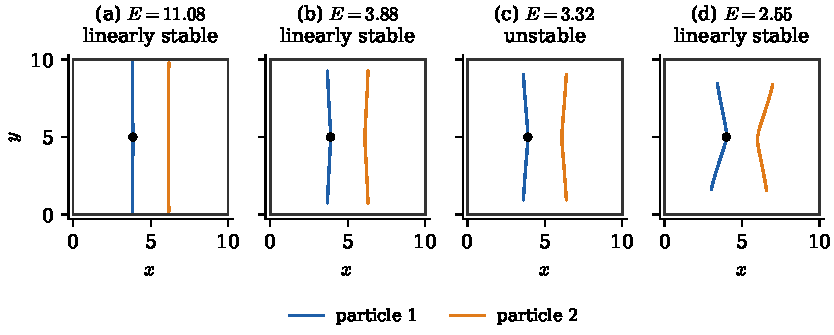
\includegraphics[width=\textwidth]{fig_vertical_family.pdf}
  \caption{Periodic orbits at four energies, obtained by continuing the vertical orbit towards lower energies. (a), (b) stable;
  (c) unstable; (d) at $E\approx2.55$ Newton found a different orbit which is curved.
  The black dot is where the orbit crosses the section $y_1=5$.}
  \label{fig:vertical}
\end{figure}

\subsection{The circular orbit}\label{app:circular}
In this orbit the two particles go round the centre of the box, always opposite
each other. We found it near the trajectory of Case~3
(Appendix~\ref{app:cases}), using the diagonal $x_1=y_1$ as the Poincar\'e section, and
followed it upward in energy (Figure~\ref{fig:circular}). Newton converged at
all 21 energies from $E\approx2.01$ to $4.02$, and every orbit found is
linearly stable; as the energy increases, the loop grows towards the walls. At
$E\approx52$ and $E\approx202$ it approaches a diamond-shaped orbit with turning points near the middle of each wall. The two particles follow the same curve half a period apart,
so this is also a choreographic motion in the terminology
of \cite{turaev2022}.

Following the orbit to energies below that of Case~3 did not work: Newton
jumped between different periodic orbits that lie close together (the period
jumped from $101.8$ to $109.2$, $135.4$ and $140.6$ with energy steps of only
$0.1\%$).
A continuation method designed to stay on one branch, such as
pseudo-arclength continuation \cite{kuznetsov}, would be needed.

\begin{figure}
  \centering
  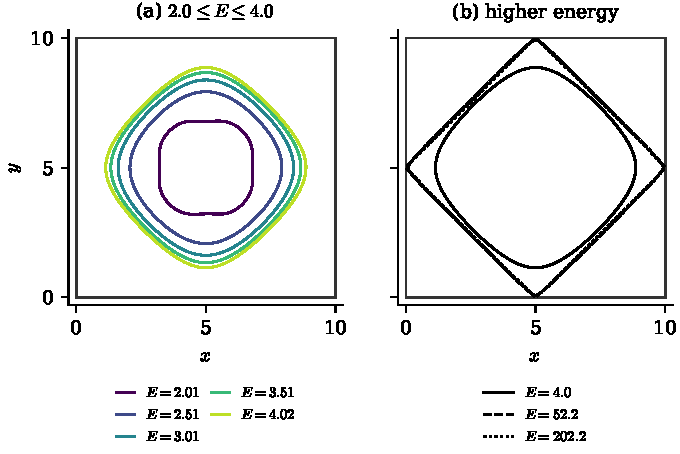
\includegraphics[width=0.8\textwidth]{fig_circular_family.pdf}
  \caption{One period of the circular orbit at several energies. The two
  particles move on the same curve, half a period apart. (a) For
  $2.0\le E\le4.0$ the loop grows towards the walls. (b) At $E\approx52$ and
  $202$ it approaches a diamond-shaped billiard orbit near all four walls. All orbits shown are linearly stable.}
  \label{fig:circular}
\end{figure}

\section{Five example trajectories}\label{app:cases}
Table~\ref{tab:cases} lists five initial conditions from the early part of
the project, and Figure~\ref{fig:cases} shows their trajectories and
Poincar\'e sections (integrated with $h=10^{-2}$ for Cases~1--3 and $10^{-4}$
for Cases~4--5).
\begin{itemize}
  \item Cases~1 and~2 start near the equilibrium and stay near it. Their
        section points lie on smooth curves, so the motion is regular.
  \item In Case~3 the particles go round the centre of the box, always
        opposite each other. The section points form two tiny clusters, which
        suggests a periodic orbit nearby (the circular orbit of
        Appendix~\ref{app:circular}).
  \item In Case~4 each particle bounces between the top and bottom walls along
        an almost vertical line. This is a periodic orbit: after one period
        $T\approx1.0027$ the state returns to its starting value to within
        $6\times10^{-7}$.
  \item Case~5 starts like Case~4 but at a different $x$. Its section points
        lie on a closed curve around the Case~4 point: the orbit oscillates
        around the stable periodic orbit of Case~4.
\end{itemize}

\begin{table}
\centering
\caption{Initial conditions. Particle~2 always starts at the point reflection
of particle~1 through the centre, with the opposite momentum. $a\approx3.6645$
is the equilibrium position.}
\vspace{1em}
\label{tab:cases}
\begin{tabular}{@{}lllll@{}}
\toprule
Case & $\q_1(0)$ & $\p_1(0)$ & $E$ & Motion\\
\midrule
1 & $(a,a)+5\cdot10^{-4}(1,1)$ & $(10^{-3},0)$ & $1.9877$ & small regular oscillation\\
2 & $(a,a)+0.25\,(1,1)$ & $(0,0.05)$ & $2.0073$ & regular\\
3 & $(a,a)+5\cdot10^{-4}(1,1)$ & $(0.1,-0.1)$ & $2.0077$ & close to a periodic loop\\
4 & $(3.8352,\,5)$ & $(0,20)$ & $402.08$ & periodic, vertical bouncing\\
5 & $(3,\,5)$ & $(0,20)$ & $402.00$ & regular, around Case 4\\
\bottomrule
\end{tabular}
\end{table}

\begin{figure}
  \centering
  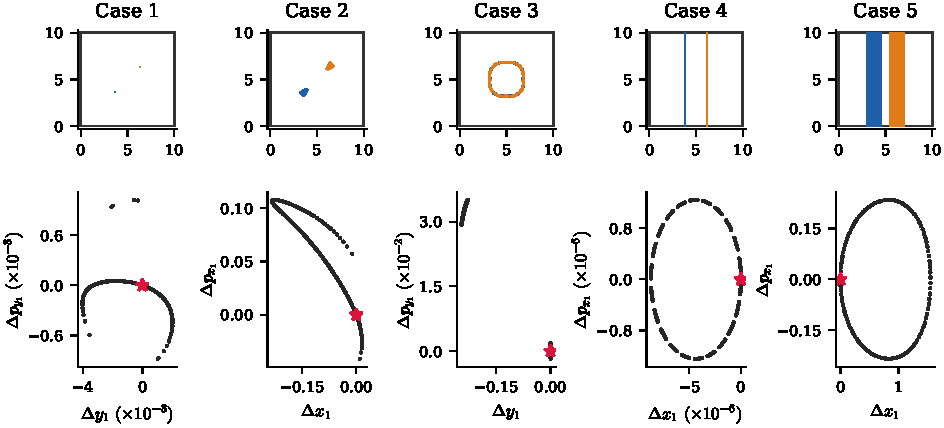
\includegraphics[width=\textwidth]{fig_cases.pdf}
  \caption{Top: trajectories of the five cases (particle~1 blue, particle~2
  orange). Bottom: 200 returns to a Poincar\'e section, measured from the
  starting point (red star). The section is taken through the starting point,
  across the largest initial velocity component of particle~1: $x_1=x_1(0)$,
  $p_{x_1}>0$ for Cases~1 and~3, so the axes are $(\Delta y_1,\Delta p_{y_1})$;
  $y_1=y_1(0)$, $p_{y_1}>0$ for Cases~2, 4 and~5, so the axes are
  $(\Delta x_1,\Delta p_{x_1})$. Note the scales: in Case~4 all returns lie
  within $10^{-5}$ of the start.}
  \label{fig:cases}
\end{figure}

% ---------------------------------------------------------------------------
\section*{Code and reproducibility}
All code is available at
\url{https://github.com/jiajunwu1729/2particle-numerics}; its README lists
the script that produces each figure and number in this report.

\section*{Acknowledgements}
I thank Prof.\ Dmitry Turaev for suggesting this project and for his guidance.

% ---------------------------------------------------------------------------
\begin{thebibliography}{9}
\bibitem{turaev2022}
V.~Rom-Kedar and D.~Turaev,
Stable motions of high energy particles interacting via a repelling potential,
\emph{Comm.\ Math.\ Phys.}\ \textbf{405} (2024), no.~6, 150;
arXiv:2208.14993.
% Verified via Crossref, DOI 10.1007/s00220-024-04946-3 (2026-11-08).

\bibitem{hairer2006}
E.~Hairer, C.~Lubich and G.~Wanner,
\emph{Geometric Numerical Integration}, 2nd ed., Springer, 2006.

\bibitem{lichtenberg1992}
A.~J.~Lichtenberg and M.~A.~Lieberman,
\emph{Regular and Chaotic Dynamics}, 2nd ed., Springer, 1992.

\bibitem{kuznetsov}
Yu.~A.~Kuznetsov, \emph{Elements of Applied Bifurcation Theory}, 3rd ed.,
Springer, 2004.
\end{thebibliography}

\end{document}
